%-----------------------------------------------------------------------
% Bericht - Vorlage für Elektrotechnik / Informationstechnik
%                         2023 HTL Weiz
%-----------------------------------------------------------------------
% Dieses LaTeX Template kann als Grundlage für die Erstellung von
% Berichten verwendet werden. In diesem File werden die Inhalte
% (Text, Bilder, Formeln, Tabellen, etc.) eingefügt und erstellt. 
%
% Im beiliegenden labstyle.sty dem sogenannten Style-File wird das 
% Aussehen und Format definiert. Des Weiteren werden in diesem File
% alle verwendeten Pakete eingebunden. 
%-----------------------------------------------------------------------

% Dokumenttyp muss hier definiert werden
\documentclass[12pt,a4paper,ngerman]{article}

% Style-File einbinden
\usepackage{labstyle} 


\begin{document}
%\pagestyle{empty}


%%%%%%%%%%%%%%%%%%%%%%%%%%%%%%%%%%%%%%%%%%%%%%%%%
%% AUFGABE 1 %%%%%%%%%%%%%%%%%%%%%%%%%%%%%%%%%%%%
%% Betreuer, Schüler, Tag, Datum, etc ergänzen 
%%%%%%%%%%%%%%%%%%%%%%%%%%%%%%%%%%%%%%%%%%%%%%%%%
%---------------------------------------------------------
\HTLheader                         				% Definierter Befehl aus .sty
{Elektrotechnisches Labor}							% #1 Labor/Fach/Titel angeben z.B. CPE
{Übung 1 \\ Messen von Strom und Spannung}   	% #2 Titel der Laborübung angeben 
{Übungsdatum: 05.03.2023}                      	% #3 Übungsdatum, Ort,... 	
{Gruppe: 2}                            			% #4 Gruppen Nr.
{Teilnehmer/innen:}								% #5 Teilnehmer/innen 
{												% #6 Übungsteilnehmer
1.~Schüler(in)\\								%  ...bei <4 Teilnehmer auskommentieren mit 
2.~Schüler(in)\\                    
3.~Schüler(in)\\                    
4.~Schüler(in)\\
}
{Betreuer: Prof. }                      		% #7 Betreuer angeben

%----------------------------------------------------------
% Inhaltsverzeichnis
%
%\frontmatter
\tableofcontents            % Legt automatisch ein Inhaltsverzeichnis an
%----------------------------------------------------------
\clearpage
%\pagestyle{fancy}
%
% Titel der Übung
\section{Messen von Strom und Spannung }

\subsection{Aufgabenstellung}
Mit einer geeigneten Messschaltung sollen an einem mit Gleichspannung versorgten unbekannten Widerstand Strom und Spannung messtechnisch erfasst werden. Diese Messung soll in vier unterschiedlichen Arbeitspunkten des Widerstands, also bei vier unterschiedlichen Werten für die Versorgungsspannung durchgeführt werden. Für jeden Arbeitspunkt ist der Wert des ohmschen Widerstands sowie die am Widerstand umgesetzte Leistung zu bestimmen.
Die Messwerte sind in einem Spannungs-Strom-Diagramm $U_R=f(I_A)$ darzustellen. In zwei weiteren Diagrammen sollen die errechneten Werte für den Widerstandswert und die Leistung als Funktion des Stroms ($R=f(I_A)$,
$P_R=f(I_A)$) grafisch präsentiert und diskutiert werden. 

\subsection{Schaltung}
Abbildung~\ref{fig:schaltbild} zeigt die Schaltung zur Strom- und Spannungsmessung an einem unbekannten Widerstand $R$ (spannungsrichtige Schaltung). Die Schaltung wird von einer Spannungsquelle mit der Spannung $U$ gespeist.

\begin{figure}[!ht]
	\begin{center}
		\includegraphics[width=0.3\textwidth]{./../03_PICS/schaltbild}
		\caption{Schaltung zur Strom- und Spannungsmessung an einem ohmschen Widerstand.} \label{fig:schaltbild}
	\end{center}
\end{figure}

\vspace{-0.5cm}


%---------- BEGIN  B l o c k   G r a p h i k  in  S u b s e c t i o n 
\begin{figure}[h!]
	\begin{minipage}{0.2\textwidth}
		\begin{center}
		\vspace{-0.0cm}\includegraphics[width=0.9\textwidth]{./../03_PICS/Prot_A_Pic_02}
		\end{center}
	\end{minipage}%\hfill
	\begin{minipage}{0.8\textwidth}
		%\linespread {1.25}\changefont{pag}{m}{n}
		Das ist irgendein Text, der in einer Spalte neben einer Grafik steht. Das ist irgendein Text, der in einer Spalte neben einer Grafik steht. Das ist irgendein Text, der in einer Spalte neben einer Grafik steht.\\
		\caption{Irgendeine Bildunterschrift.}
		\label{fig:Prot_A_Pic_02}	
	\end{minipage}
\end{figure}
%---------- END  B l o c k   G r a p h i k  in  S u b s e c t i o n
%%%%%%%%%%%%%%%%%%%%%%%%%%%%%%%%%%%%%%%%%%%%%%%%%
%% AUFGABE 4 %%%%%%%%%%%%%%%%%%%%%%%%%%%%%%%%%%%%
%% HIER DIE NEUE REFERENZ EINBINDEN 
%% (ZUERST MUSS DIESE IN htllab.bib ERGÄNZT WERDEN)
%%%%%%%%%%%%%%%%%%%%%%%%%%%%%%%%%%%%%%%%%%%%%%%%%


\subsection{Tabellen}
%
Tabelle~\ref{tab:messwerte} zeigt die an der Spannungsquelle eingestellten Werte $U$ sowie die gemessenen Werte für Strom $I_A$ und Spannung $U_R$ für alle durchgeführten Messungen. Die errechneten Werte für den Widerstand $R$ sowie die umgesetzte Leistung $P_R$ sind anschließend an die Messwerte in der Tabelle angegeben.

\pagebreak
\begin{table}[!htp]
	\begin{center}
		\begin{tabular}
			{| c || c || c | c || c | c |}   %  || zur Unterteilung eingestellte/gemnessene/berechnete Werte
			\hline
			\multicolumn{2}{|c||}{Eingestellt} &
			\multicolumn{2}{c||}{Gemessen} &
			\multicolumn{2}{c|}{Berechnet} \\ \hline
			Messung & $U$ & $U_{R}$  & $I_{A}$& $R$      & $P_R$     \\ \hline
			Nr.     &  V  &  V       &  mA    & $\Omega$ &  mW       \\ \hline\hline
			1       & 4,00&  4,01    & 1,01   &  3970    &  4,05     \\ \hline
			2       & 8,00&  7,73    & 1,93   &  4005    &  14,92    \\ \hline
			3       &12,00& 12,22    & 3,05   &  4007    &  37,27    \\ \hline
			4       &16,00& 15,92    & 3,97   &  4010    &  63,20    \\
			\hline
		\end{tabular}
		\caption{Eingestellte, gemessene und berechnete Werte.\label{tab:messwerte}}
	\end{center}
\end{table}

\subsection{Formeln}
%
Bei Versorgung mit Gleichspannung kann der ohmsche Widerstand $R$ aus den gemessenen Werten von Strom $I_A$ und Spannung $U_R$ wie folgt berechnet werden:
\begin{equation}\label{eq:widerstand}
	R = \frac{U_R}{I_A}\,.
\end{equation}
Die dabei im ohmschen Verbraucher umgesetzte Leistung erhält man nach 

%%%%%%%%%%%%%%%%%%%%%%%%%%%%%%%%%%%%%%%%%%
%% AUFGABE 2 %%%%%%%%%%%%%%%%%%%%%%%%%%%%%
%% HIER DIE FORMEL UND BERECHNUNG ERGÄNZEN
%%%%%%%%%%%%%%%%%%%%%%%%%%%%%%%%%%%%%%%%%%

\subsection{Berechnungsbeispiele}
%
Für eine an der Spannungsquelle eingestellte Spannung von $U=8\,$V erhält man den Widerstandswert $R$ aus den zugehörigen Messwerten aus Tabelle~\ref{tab:messwerte} zu
\begin{equation}\label{eq:bsp_widerstand}
	R = \frac{U_R}{I_A}=\frac{7,73\,\mathrm{V}}{1,93\cdot10^{-3}\,\mathrm{A}}= 4005\,\Omega\,.
\end{equation}
Die im Widerstand umgesetzte Wirkleistung berechnet man aus den gemessenen Werten zu
\begin{equation}\label{eq:bsp_leistung}
	P_R = {U_R}\cdot{I_A}={7,73\,\mathrm{V}}\cdot{1,93\cdot10^{-3}\,\mathrm{A}}=
	14,92\cdot10^{-3}\,\mathrm{W}= 14,92\,\mathrm{mW}\,.
\end{equation}

\subsection{Diagramme}
%
Die folgenden Diagramme wurden erstellt:

\begin{enumerate}
	\item Spannung als Funktion des Stroms U = f(I)
	\item Widerstand als Funktion des Stroms R = f(I)
	\item Leistung als Funktion des Stroms P = f(I)
\end{enumerate}

Das Diagramm in Abb.~\ref{fig:spannungstrom} zeigt den aus den
Messwerten ermittelten Zusammenhang zwischen $U_R$ und $I_A$.

Abb.~\ref{fig:widerstand} zeigt den Verlauf des errechneten Widerstandswertes $R$ als Funktion des gemessenen Stroms $I_A$.

In Abb.~\ref{fig:leistung} erkennt man den quadratischen Zusammenhang zwischen dem Strom $I_A$ und der im ohmschen Widerstand umgesetzten Leistung $P_R$. Dieser Zusammenhang wurde auch anhand des Lehrbuches \cite{Buch:Deimel1} vorab besprochen. \cite{unbehauen2013elektrische}

%
\pagebreak

\begin{figure}[!ht]
	\begin{center}
		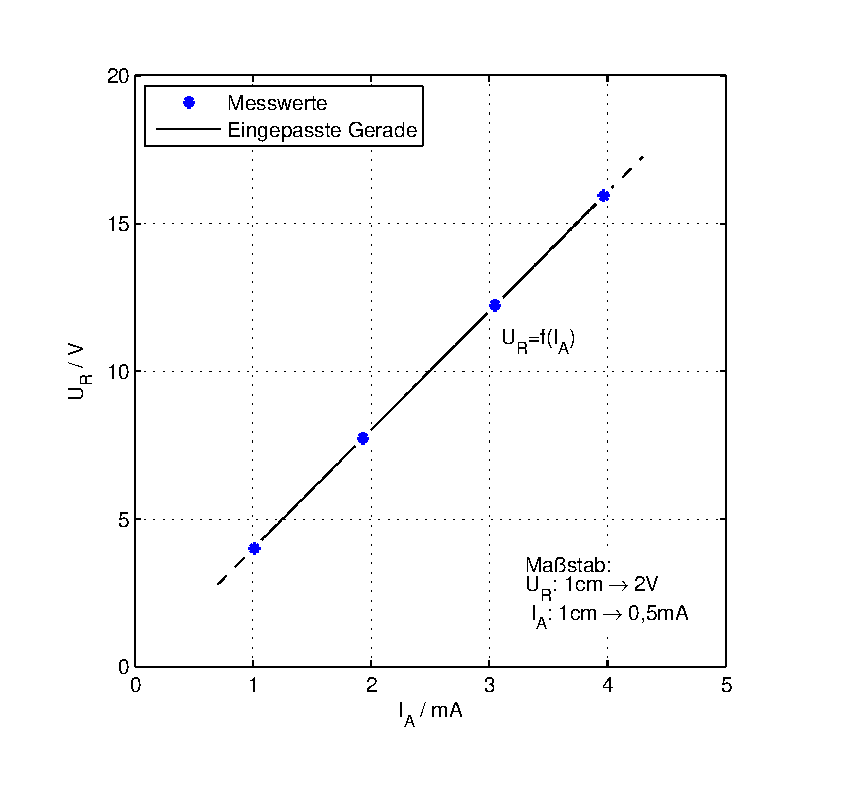
\includegraphics{./../03_PICS/spannungstrom}\vspace*{-1cm}
		\caption{Messung am ohmschen Widerstand: Zusammenhang zwischen
			Strom und Spannung.}
		\label{fig:spannungstrom}
	\end{center}
\end{figure}

\begin{figure}[!ht]
	\begin{center}
		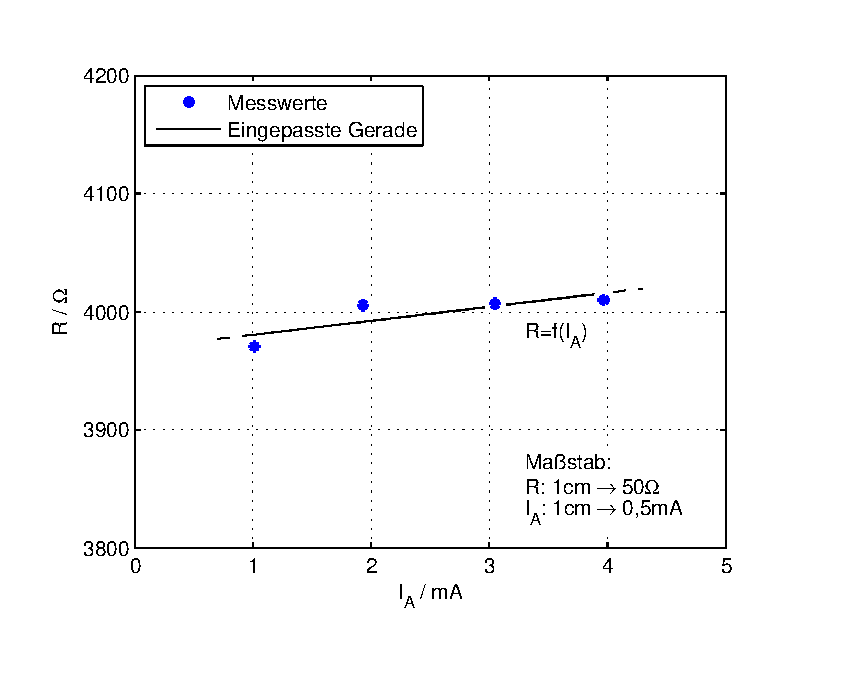
\includegraphics{./../03_PICS/widerstand}\vspace*{-1cm}
		\caption{Berechneter Widerstandswert als Funktion des gemessenen Stroms.}
		\label{fig:widerstand}
	\end{center}
\end{figure}

%%%%%%%%%%%%%%%%%%%%%%%%%%%%%%%%%%%%%%%%%%%%%%%%%
%% AUFGABE 3 %%%%%%%%%%%%%%%%%%%%%%%%%%%%%%%%%%%%
%% HIER DIE GRAPHIK "leistung" EINBINDEN 
%%%%%%%%%%%%%%%%%%%%%%%%%%%%%%%%%%%%%%%%%%%%%%%%%


%\clearpage  % damit alle Diagramme vor der Diskussion und dem Geräteverzeichnis platziert werden

\subsection{Diskussion}
%
An einem idealen ohmschen Widerstand ergibt sich ein linearer Zusammenhang
zwischen Strom und Spannung, gegeben durch den konstanten Widerstandswert.
Die geringfügigen Abweichungen der gemessenen Werte vom idealen Verlauf in Abb.~\ref{fig:spannungstrom} lassen sich durch Messunsicherheiten erklären.

Der konstante Widerstandswert des Versuchsobjekts ist in Abb.~\ref{fig:widerstand} als Funktion des gemessenen Stroms dargestellt. Es ergeben sich geringfügige
Abweichungen vom idealen konstanten Wert, die gewählte Darstellung im Bereich von
$R=3800\Omega\dots4200\Omega$ verdeutlicht die Abweichung der errechneten Werte vom konstanten Idealwert.

Für einen ohmschen Widerstand stellt sich ein quadratischer Zusammenhang zwischen der umgesetzten Wirkleistung und dem durchfließenden Strom ein, wie in~\cite{Skript:ES1} diskutiert. Die ermittelten Leistungswerte liegen sehr nahe am eingepassten Polynom 2. Ordnung, wie in Abb.~\ref{fig:leistung} ersichtlich.

\subsection{Geräteverzeichnis}
%
1Stk. Leistungswiderstand Nr. 16, Aufgedruckter Wert: 4$\,$k$\Omega$.\\
1Stk. Netzgerät Type HP 6136A, S/N: 100X3499.\\
1Stk. Digitales Multimeter Fluke 87, S/N: 12F346, TRMS.\\
1Stk. Digitales Multimeter Fluke 79, S/N: D45X99.\\

%%%%%%%%%%%%%%%%%%%%%%%%%%%%%%%%%%%%%%%%%%%%%%%%%
%% AUFGABE 5 %%%%%%%%%%%%%%%%%%%%%%%%%%%%%%%%%%%%
%% GERÄTEVERZEICHNIS IN EINER TABELLE DARSTELLEN
%%%%%%%%%%%%%%%%%%%%%%%%%%%%%%%%%%%%%%%%%%%%%%%%%


%\section{Übung~2: \dots}   % Weitere unabhängige Teilübungen
%
%\vspace*{2cm}
% \section*{Unterschriften der Übungsteilnehmer}   % aktivieren bei Protokollabgabe in Papierform 
%
\vspace*{1cm}
%
Autor in Blockbuchstaben:\\					% Ersteller des Berichts		 
Unterschrift: 								% Unterschriften auf Ausdruck!
%
\vspace*{1cm}
%
%-----------------------------------------------
% Bibliographie, wenn notwendig. 
% Ansonsten: Auskommentieren!
%
\bibliographystyle{unsrt} 		%Sortiert die Reihenfolge der Literaturstellen nach Verwendungsreihenfolge
\bibliography{htllab}
\end{document}
